\documentclass[twoside]{book}

% Packages required by doxygen
\usepackage{fixltx2e}
\usepackage{calc}
\usepackage{doxygen}
\usepackage[export]{adjustbox} % also loads graphicx
\usepackage{graphicx}
\usepackage[utf8]{inputenc}
\usepackage{makeidx}
\usepackage{multicol}
\usepackage{multirow}
\PassOptionsToPackage{warn}{textcomp}
\usepackage{textcomp}
\usepackage[nointegrals]{wasysym}
\usepackage[table]{xcolor}

% Font selection
\usepackage[T1]{fontenc}
\usepackage[scaled=.90]{helvet}
\usepackage{courier}
\usepackage{amssymb}
\usepackage{sectsty}
\renewcommand{\familydefault}{\sfdefault}
\allsectionsfont{%
  \fontseries{bc}\selectfont%
  \color{darkgray}%
}
\renewcommand{\DoxyLabelFont}{%
  \fontseries{bc}\selectfont%
  \color{darkgray}%
}
\newcommand{\+}{\discretionary{\mbox{\scriptsize$\hookleftarrow$}}{}{}}

% Page & text layout
\usepackage{geometry}
\geometry{%
  a4paper,%
  top=2.5cm,%
  bottom=2.5cm,%
  left=2.5cm,%
  right=2.5cm%
}
\tolerance=750
\hfuzz=15pt
\hbadness=750
\setlength{\emergencystretch}{15pt}
\setlength{\parindent}{0cm}
\setlength{\parskip}{3ex plus 2ex minus 2ex}
\makeatletter
\renewcommand{\paragraph}{%
  \@startsection{paragraph}{4}{0ex}{-1.0ex}{1.0ex}{%
    \normalfont\normalsize\bfseries\SS@parafont%
  }%
}
\renewcommand{\subparagraph}{%
  \@startsection{subparagraph}{5}{0ex}{-1.0ex}{1.0ex}{%
    \normalfont\normalsize\bfseries\SS@subparafont%
  }%
}
\makeatother

% Headers & footers
\usepackage{fancyhdr}
\pagestyle{fancyplain}
\fancyhead[LE]{\fancyplain{}{\bfseries\thepage}}
\fancyhead[CE]{\fancyplain{}{}}
\fancyhead[RE]{\fancyplain{}{\bfseries\leftmark}}
\fancyhead[LO]{\fancyplain{}{\bfseries\rightmark}}
\fancyhead[CO]{\fancyplain{}{}}
\fancyhead[RO]{\fancyplain{}{\bfseries\thepage}}
\fancyfoot[LE]{\fancyplain{}{}}
\fancyfoot[CE]{\fancyplain{}{}}
\fancyfoot[RE]{\fancyplain{}{\bfseries\scriptsize Generated by Doxygen }}
\fancyfoot[LO]{\fancyplain{}{\bfseries\scriptsize Generated by Doxygen }}
\fancyfoot[CO]{\fancyplain{}{}}
\fancyfoot[RO]{\fancyplain{}{}}
\renewcommand{\footrulewidth}{0.4pt}
\renewcommand{\chaptermark}[1]{%
  \markboth{#1}{}%
}
\renewcommand{\sectionmark}[1]{%
  \markright{\thesection\ #1}%
}

% Indices & bibliography
\usepackage{natbib}
\usepackage[titles]{tocloft}
\setcounter{tocdepth}{3}
\setcounter{secnumdepth}{5}
\makeindex

% Hyperlinks (required, but should be loaded last)
\usepackage{ifpdf}
\ifpdf
  \usepackage[pdftex,pagebackref=true]{hyperref}
\else
  \usepackage[ps2pdf,pagebackref=true]{hyperref}
\fi
\hypersetup{%
  colorlinks=true,%
  linkcolor=blue,%
  citecolor=blue,%
  unicode%
}

% Custom commands
\newcommand{\clearemptydoublepage}{%
  \newpage{\pagestyle{empty}\cleardoublepage}%
}

\usepackage{caption}
\captionsetup{labelsep=space,justification=centering,font={bf},singlelinecheck=off,skip=4pt,position=top}

%===== C O N T E N T S =====

\begin{document}

% Titlepage & ToC
\hypersetup{pageanchor=false,
             bookmarksnumbered=true,
             pdfencoding=unicode
            }
\pagenumbering{alph}
\begin{titlepage}
\vspace*{7cm}
\begin{center}%
{\Large Nautical }\\
\vspace*{1cm}
{\large Generated by Doxygen 1.8.13}\\
\end{center}
\end{titlepage}
\clearemptydoublepage
\pagenumbering{roman}
\tableofcontents
\clearemptydoublepage
\pagenumbering{arabic}
\hypersetup{pageanchor=true}

%--- Begin generated contents ---
\chapter{Class Index}
\section{Data Structures}
Here are the data structures with brief descriptions\+:\begin{DoxyCompactList}
\item\contentsline{section}{\hyperlink{structahrs}{ahrs} }{\pageref{structahrs}}{}
\item\contentsline{section}{\hyperlink{structdvl__data}{dvl\+\_\+data} }{\pageref{structdvl__data}}{}
\item\contentsline{section}{\hyperlink{structKalman}{Kalman} \\*Struct to make using the \hyperlink{structKalman}{Kalman} filter easier }{\pageref{structKalman}}{}
\item\contentsline{section}{\hyperlink{structMotors}{Motors} \\*Helper class for motors }{\pageref{structMotors}}{}
\item\contentsline{section}{\hyperlink{structparser__var__t}{parser\+\_\+var\+\_\+t} }{\pageref{structparser__var__t}}{}
\item\contentsline{section}{\hyperlink{structPID}{P\+ID} \\*Helper class for \hyperlink{structPID}{P\+ID} computations }{\pageref{structPID}}{}
\item\contentsline{section}{\hyperlink{structservo__t}{servo\+\_\+t} }{\pageref{structservo__t}}{}
\item\contentsline{section}{\hyperlink{classServoArrayT2}{Servo\+Array\+T2} }{\pageref{classServoArrayT2}}{}
\item\contentsline{section}{\hyperlink{structServoPin__t}{Servo\+Pin\+\_\+t} }{\pageref{structServoPin__t}}{}
\item\contentsline{section}{\hyperlink{classServoTimer2}{Servo\+Timer2} }{\pageref{classServoTimer2}}{}
\end{DoxyCompactList}

\chapter{File Index}
\section{File List}
Here is a list of all documented files with brief descriptions\+:\begin{DoxyCompactList}
\item\contentsline{section}{include/\hyperlink{config_8h}{config.\+h} \\*Configuration options for Nautical }{\pageref{config_8h}}{}
\item\contentsline{section}{include/\hyperlink{dbg_8h}{dbg.\+h} \\*Debug functions for A\+VR }{\pageref{dbg_8h}}{}
\item\contentsline{section}{include/\hyperlink{io_8hpp}{io.\+hpp} \\*IO and kill switch function definitions }{\pageref{io_8hpp}}{}
\item\contentsline{section}{include/\hyperlink{kalman_8hpp}{kalman.\+hpp} \\*\hyperlink{structKalman}{Kalman} filter struct and constant definitions }{\pageref{kalman_8hpp}}{}
\item\contentsline{section}{include/\hyperlink{macrodef_8h}{macrodef.\+h} \\*Helper macros for various parts of Nautical }{\pageref{macrodef_8h}}{}
\item\contentsline{section}{include/\hyperlink{matrix_8h}{matrix.\+h} \\*Function declarations for matrix operations }{\pageref{matrix_8h}}{}
\item\contentsline{section}{include/\hyperlink{motor_8hpp}{motor.\+hpp} \\*Helper class to use all of the motors at once and do computations }{\pageref{motor_8hpp}}{}
\item\contentsline{section}{include/\hyperlink{pid_8hpp}{pid.\+hpp} \\*Helper class to compute \hyperlink{structPID}{P\+ID} for motors }{\pageref{pid_8hpp}}{}
\item\contentsline{section}{include/{\bfseries rotation.\+h} }{\pageref{rotation_8h}}{}
\item\contentsline{section}{include/{\bfseries util.\+hpp} }{\pageref{util_8hpp}}{}
\item\contentsline{section}{include/{\bfseries voltage.\+hpp} }{\pageref{voltage_8hpp}}{}
\item\contentsline{section}{include/ahrs/\hyperlink{ahrs_8h}{ahrs.\+h} \\*Interface function definitions for the A\+H\+RS }{\pageref{ahrs_8h}}{}
\item\contentsline{section}{include/ahrs/\hyperlink{crc__xmodem_8h}{crc\+\_\+xmodem.\+h} \\*Helper macros for C\+R\+C-\/\+X\+M\+O\+D\+EM updating }{\pageref{crc__xmodem_8h}}{}
\item\contentsline{section}{include/ahrs/\hyperlink{crc__xmodem__generic_8h}{crc\+\_\+xmodem\+\_\+generic.\+h} \\*C\+RC update functions for testing }{\pageref{crc__xmodem__generic_8h}}{}
\item\contentsline{section}{include/ahrs/\hyperlink{io__ahrs_8h}{io\+\_\+ahrs.\+h} \\*Low-\/level communication function definitions for A\+H\+RS }{\pageref{io__ahrs_8h}}{}
\item\contentsline{section}{include/dvl/\hyperlink{dvl_8h}{dvl.\+h} \\*Interface function definitions for D\+VL }{\pageref{dvl_8h}}{}
\item\contentsline{section}{include/dvl/\hyperlink{dvl__commands_8h}{dvl\+\_\+commands.\+h} \\*Interface function definitions for D\+VL }{\pageref{dvl__commands_8h}}{}
\item\contentsline{section}{include/dvl/\hyperlink{io__dvl_8h}{io\+\_\+dvl.\+h} \\*Low-\/level communication function definitions for D\+VL }{\pageref{io__dvl_8h}}{}
\item\contentsline{section}{include/m5/\hyperlink{crc32_8h}{crc32.\+h} \\*Helper functions for C\+RC }{\pageref{crc32_8h}}{}
\item\contentsline{section}{include/m5/\hyperlink{io__m5_8h}{io\+\_\+m5.\+h} \\*Low-\/level communication function definitions for Videoray M5 motors }{\pageref{io__m5_8h}}{}
\item\contentsline{section}{include/m5/\hyperlink{m5_8h}{m5.\+h} \\*Interface function definitions for Videoray M5 motors }{\pageref{m5_8h}}{}
\end{DoxyCompactList}

\chapter{Class Documentation}
\hypertarget{struct__BASED}{}\section{\+\_\+\+B\+A\+S\+ED Struct Reference}
\label{struct__BASED}\index{\+\_\+\+B\+A\+S\+ED@{\+\_\+\+B\+A\+S\+ED}}
\subsection*{Public Member Functions}
\begin{DoxyCompactItemize}
\item 
\mbox{\Hypertarget{struct__BASED_ad245ef70c87f1b0680451c69e84d9a86}\label{struct__BASED_ad245ef70c87f1b0680451c69e84d9a86}} 
{\bfseries \+\_\+\+B\+A\+S\+ED} (long v, int b)
\end{DoxyCompactItemize}
\subsection*{Public Attributes}
\begin{DoxyCompactItemize}
\item 
\mbox{\Hypertarget{struct__BASED_a9aa9980a497acaa8856a0d0572f13191}\label{struct__BASED_a9aa9980a497acaa8856a0d0572f13191}} 
long {\bfseries val}
\item 
\mbox{\Hypertarget{struct__BASED_a2d2f682a027ec75d3c5c3e365d9325f0}\label{struct__BASED_a2d2f682a027ec75d3c5c3e365d9325f0}} 
int {\bfseries base}
\end{DoxyCompactItemize}


The documentation for this struct was generated from the following file\+:\begin{DoxyCompactItemize}
\item 
include/streaming.\+h\end{DoxyCompactItemize}

\hypertarget{structKalman}{}\section{Kalman Struct Reference}
\label{structKalman}\index{Kalman@{Kalman}}


Struct to make using the \hyperlink{structKalman}{Kalman} filter easier.  




{\ttfamily \#include $<$kalman.\+hpp$>$}

\subsection*{Public Member Functions}
\begin{DoxyCompactItemize}
\item 
\mbox{\Hypertarget{structKalman_a92d8a2bf6c725e8ad7da1015bbc41cdc}\label{structKalman_a92d8a2bf6c725e8ad7da1015bbc41cdc}} 
void \hyperlink{structKalman_a92d8a2bf6c725e8ad7da1015bbc41cdc}{bias} ()
\begin{DoxyCompactList}\small\item\em Removes bias from accelerometer data. \end{DoxyCompactList}\item 
uint32\+\_\+t \hyperlink{structKalman_ab314838fbb97199c19cd0fb48fffcfc4}{compute} (float $\ast$state, float $\ast$covar, float $\ast$angles, uint32\+\_\+t t)
\begin{DoxyCompactList}\small\item\em Computes one iteration of the \hyperlink{structKalman}{Kalman} filter. \end{DoxyCompactList}\end{DoxyCompactItemize}
\subsection*{Data Fields}
\textbf{ }\par
\begin{DoxyCompactItemize}
\item 
int \hyperlink{structKalman_a79ded01709506f54e5e2ef5d0b1c5ddf}{skip}
\item 
int \hyperlink{structKalman_a98fa8a7387b5714f1f5d9d85a2555411}{iter}
\item 
float \hyperlink{structKalman_a1672e563d4e6cc8f23b3fb4d1c546fe8}{m\+\_\+orig} \mbox{[}M\mbox{]}
\item 
float \hyperlink{structKalman_ace399cd36d8df2e905562b5d0952d11f}{m\+\_\+bias} \mbox{[}M\mbox{]}
\end{DoxyCompactItemize}



\subsection{Detailed Description}
Struct to make using the \hyperlink{structKalman}{Kalman} filter easier. 

\subsection{Member Function Documentation}
\mbox{\Hypertarget{structKalman_ab314838fbb97199c19cd0fb48fffcfc4}\label{structKalman_ab314838fbb97199c19cd0fb48fffcfc4}} 
\index{Kalman@{Kalman}!compute@{compute}}
\index{compute@{compute}!Kalman@{Kalman}}
\subsubsection{\texorpdfstring{compute()}{compute()}}
{\footnotesize\ttfamily uint32\+\_\+t Kalman\+::compute (\begin{DoxyParamCaption}\item[{float $\ast$}]{state,  }\item[{float $\ast$}]{covar,  }\item[{float $\ast$}]{angles,  }\item[{uint32\+\_\+t}]{t }\end{DoxyParamCaption})}



Computes one iteration of the \hyperlink{structKalman}{Kalman} filter. 


\begin{DoxyParams}{Parameters}
{\em state} & The current state of the sub using the \hyperlink{structKalman}{Kalman} state model. \\
\hline
{\em covar} & The current error of the state. \\
\hline
{\em angles} & The current euler angles of the sub. \\
\hline
{\em t} & The current time of system, used to compute time differences. \\
\hline
\end{DoxyParams}
\begin{DoxyReturn}{Returns}
The end time of the system. 
\end{DoxyReturn}


\subsection{Field Documentation}
\mbox{\Hypertarget{structKalman_a98fa8a7387b5714f1f5d9d85a2555411}\label{structKalman_a98fa8a7387b5714f1f5d9d85a2555411}} 
\index{Kalman@{Kalman}!iter@{iter}}
\index{iter@{iter}!Kalman@{Kalman}}
\subsubsection{\texorpdfstring{iter}{iter}}
{\footnotesize\ttfamily int Kalman\+::iter}

Supposed to be used for accelerometer bias removal, unused for now. \mbox{\Hypertarget{structKalman_ace399cd36d8df2e905562b5d0952d11f}\label{structKalman_ace399cd36d8df2e905562b5d0952d11f}} 
\index{Kalman@{Kalman}!m\+\_\+bias@{m\+\_\+bias}}
\index{m\+\_\+bias@{m\+\_\+bias}!Kalman@{Kalman}}
\subsubsection{\texorpdfstring{m\+\_\+bias}{m\_bias}}
{\footnotesize\ttfamily float Kalman\+::m\+\_\+bias\mbox{[}M\mbox{]}}

Supposed to be used for accelerometer bias removal, unused for now. \mbox{\Hypertarget{structKalman_a1672e563d4e6cc8f23b3fb4d1c546fe8}\label{structKalman_a1672e563d4e6cc8f23b3fb4d1c546fe8}} 
\index{Kalman@{Kalman}!m\+\_\+orig@{m\+\_\+orig}}
\index{m\+\_\+orig@{m\+\_\+orig}!Kalman@{Kalman}}
\subsubsection{\texorpdfstring{m\+\_\+orig}{m\_orig}}
{\footnotesize\ttfamily float Kalman\+::m\+\_\+orig\mbox{[}M\mbox{]}}

Supposed to be used for accelerometer bias removal, unused for now. \mbox{\Hypertarget{structKalman_a79ded01709506f54e5e2ef5d0b1c5ddf}\label{structKalman_a79ded01709506f54e5e2ef5d0b1c5ddf}} 
\index{Kalman@{Kalman}!skip@{skip}}
\index{skip@{skip}!Kalman@{Kalman}}
\subsubsection{\texorpdfstring{skip}{skip}}
{\footnotesize\ttfamily int Kalman\+::skip}

Supposed to be used for accelerometer bias removal, unused for now. 

The documentation for this struct was generated from the following files\+:\begin{DoxyCompactItemize}
\item 
include/\hyperlink{kalman_8hpp}{kalman.\+hpp}\item 
src/kalman.\+cpp\end{DoxyCompactItemize}

\hypertarget{structMotors}{}\section{Motors Struct Reference}
\label{structMotors}\index{Motors@{Motors}}


Helper class for motors.  




{\ttfamily \#include $<$motor.\+hpp$>$}



Collaboration diagram for Motors\+:
\nopagebreak
\begin{figure}[H]
\begin{center}
\leavevmode
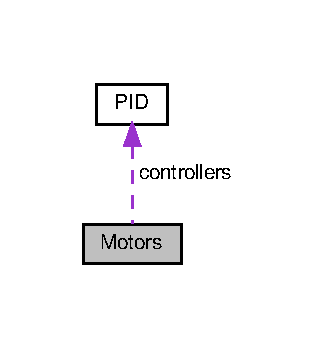
\includegraphics[width=153pt]{structMotors__coll__graph}
\end{center}
\end{figure}
\subsection*{Public Member Functions}
\begin{DoxyCompactItemize}
\item 
\mbox{\Hypertarget{structMotors_ac6532a754e5f1743ee4975b6722b4054}\label{structMotors_ac6532a754e5f1743ee4975b6722b4054}} 
void \hyperlink{structMotors_ac6532a754e5f1743ee4975b6722b4054}{power} ()
\begin{DoxyCompactList}\small\item\em Set power to the motors using the current thrust vector. \end{DoxyCompactList}\item 
\mbox{\Hypertarget{structMotors_a179c6a24115935994a13493f74f56df8}\label{structMotors_a179c6a24115935994a13493f74f56df8}} 
void \hyperlink{structMotors_a179c6a24115935994a13493f74f56df8}{pause} ()
\begin{DoxyCompactList}\small\item\em Pause power to the motors. \end{DoxyCompactList}\item 
uint32\+\_\+t \hyperlink{structMotors_a0d3909ec9fadbb3028368e7340a2e707}{run} (float $\ast$dstate, float $\ast$angles, uint32\+\_\+t t)
\begin{DoxyCompactList}\small\item\em Run the motors for one iteration towards the desired state. \end{DoxyCompactList}\end{DoxyCompactItemize}
\subsection*{Data Fields}
\begin{DoxyCompactItemize}
\item 
\hyperlink{structPID}{P\+ID} \hyperlink{structMotors_a7cbe4b9467412e4882ff318b9375017e}{controllers} \mbox{[}\hyperlink{config_8h_ab5c558d88abd9517fb657be4889ee1bc}{D\+OF}\mbox{]}
\item 
float \hyperlink{structMotors_ac8d20987287ffda85eed109c3bf80a12}{thrust} \mbox{[}\hyperlink{config_8h_ae84658f12c2f1b44f59af36678cf3dcc}{N\+U\+M\+\_\+\+M\+O\+T\+O\+RS}\mbox{]}
\item 
int \hyperlink{structMotors_a84b2ea1a929743410df7ead8212b767a}{buttons} \mbox{[}\hyperlink{config_8h_ae84658f12c2f1b44f59af36678cf3dcc}{N\+U\+M\+\_\+\+M\+O\+T\+O\+RS}\mbox{]}
\item 
float \hyperlink{structMotors_a17cb9b1c3fc7749984c4622439901f84}{forces} \mbox{[}\hyperlink{config_8h_ab5c558d88abd9517fb657be4889ee1bc}{D\+OF}\mbox{]}
\item 
float \hyperlink{structMotors_a94c46cb5dab8c60c9fae75cc6b7af629}{pid} \mbox{[}\hyperlink{config_8h_ab5c558d88abd9517fb657be4889ee1bc}{D\+OF}\mbox{]}
\item 
float \hyperlink{structMotors_a46e39ac60edebef57fca46f878e2c0b5}{p}
\end{DoxyCompactItemize}


\subsection{Detailed Description}
Helper class for motors. 

\subsection{Member Function Documentation}
\mbox{\Hypertarget{structMotors_a0d3909ec9fadbb3028368e7340a2e707}\label{structMotors_a0d3909ec9fadbb3028368e7340a2e707}} 
\index{Motors@{Motors}!run@{run}}
\index{run@{run}!Motors@{Motors}}
\subsubsection{\texorpdfstring{run()}{run()}}
{\footnotesize\ttfamily uint32\+\_\+t Motors\+::run (\begin{DoxyParamCaption}\item[{float $\ast$}]{dstate,  }\item[{float $\ast$}]{angles,  }\item[{uint32\+\_\+t}]{t }\end{DoxyParamCaption})}



Run the motors for one iteration towards the desired state. 


\begin{DoxyParams}{Parameters}
{\em dstate} & Difference between desired and current state. \\
\hline
{\em angles} & Current euler angles. \\
\hline
{\em t} & Current time used for time difference calculations. \\
\hline
\end{DoxyParams}
\begin{DoxyReturn}{Returns}
Time after iteration is finished. 
\end{DoxyReturn}


\subsection{Field Documentation}
\mbox{\Hypertarget{structMotors_a84b2ea1a929743410df7ead8212b767a}\label{structMotors_a84b2ea1a929743410df7ead8212b767a}} 
\index{Motors@{Motors}!buttons@{buttons}}
\index{buttons@{buttons}!Motors@{Motors}}
\subsubsection{\texorpdfstring{buttons}{buttons}}
{\footnotesize\ttfamily int Motors\+::buttons\mbox{[}\hyperlink{config_8h_ae84658f12c2f1b44f59af36678cf3dcc}{N\+U\+M\+\_\+\+M\+O\+T\+O\+RS}\mbox{]}}

Holds pressed values for remote control. \mbox{\Hypertarget{structMotors_a7cbe4b9467412e4882ff318b9375017e}\label{structMotors_a7cbe4b9467412e4882ff318b9375017e}} 
\index{Motors@{Motors}!controllers@{controllers}}
\index{controllers@{controllers}!Motors@{Motors}}
\subsubsection{\texorpdfstring{controllers}{controllers}}
{\footnotesize\ttfamily \hyperlink{structPID}{P\+ID} Motors\+::controllers\mbox{[}\hyperlink{config_8h_ab5c558d88abd9517fb657be4889ee1bc}{D\+OF}\mbox{]}}

\hyperlink{structPID}{P\+ID} controllers for each degree of freedom. \mbox{\Hypertarget{structMotors_a17cb9b1c3fc7749984c4622439901f84}\label{structMotors_a17cb9b1c3fc7749984c4622439901f84}} 
\index{Motors@{Motors}!forces@{forces}}
\index{forces@{forces}!Motors@{Motors}}
\subsubsection{\texorpdfstring{forces}{forces}}
{\footnotesize\ttfamily float Motors\+::forces\mbox{[}\hyperlink{config_8h_ab5c558d88abd9517fb657be4889ee1bc}{D\+OF}\mbox{]}}

Theoretical forces for each degree of freedom. \mbox{\Hypertarget{structMotors_a46e39ac60edebef57fca46f878e2c0b5}\label{structMotors_a46e39ac60edebef57fca46f878e2c0b5}} 
\index{Motors@{Motors}!p@{p}}
\index{p@{p}!Motors@{Motors}}
\subsubsection{\texorpdfstring{p}{p}}
{\footnotesize\ttfamily float Motors\+::p}

Current submarine power. \mbox{\Hypertarget{structMotors_a94c46cb5dab8c60c9fae75cc6b7af629}\label{structMotors_a94c46cb5dab8c60c9fae75cc6b7af629}} 
\index{Motors@{Motors}!pid@{pid}}
\index{pid@{pid}!Motors@{Motors}}
\subsubsection{\texorpdfstring{pid}{pid}}
{\footnotesize\ttfamily float Motors\+::pid\mbox{[}\hyperlink{config_8h_ab5c558d88abd9517fb657be4889ee1bc}{D\+OF}\mbox{]}}

Computed \hyperlink{structPID}{P\+ID} values from each controller. \mbox{\Hypertarget{structMotors_ac8d20987287ffda85eed109c3bf80a12}\label{structMotors_ac8d20987287ffda85eed109c3bf80a12}} 
\index{Motors@{Motors}!thrust@{thrust}}
\index{thrust@{thrust}!Motors@{Motors}}
\subsubsection{\texorpdfstring{thrust}{thrust}}
{\footnotesize\ttfamily float Motors\+::thrust\mbox{[}\hyperlink{config_8h_ae84658f12c2f1b44f59af36678cf3dcc}{N\+U\+M\+\_\+\+M\+O\+T\+O\+RS}\mbox{]}}

Current thrust values for each of the motors. 

The documentation for this struct was generated from the following files\+:\begin{DoxyCompactItemize}
\item 
include/\hyperlink{motor_8hpp}{motor.\+hpp}\item 
src/motor.\+cpp\end{DoxyCompactItemize}

\hypertarget{structPID}{}\section{P\+ID Struct Reference}
\label{structPID}\index{P\+ID@{P\+ID}}
\subsection*{Public Member Functions}
\begin{DoxyCompactItemize}
\item 
\mbox{\Hypertarget{structPID_ac5b3e2a5ad35e07517f40b8164821f8e}\label{structPID_ac5b3e2a5ad35e07517f40b8164821f8e}} 
{\bfseries P\+ID} (float a, float b, float c)
\item 
\mbox{\Hypertarget{structPID_a43370ace90e60c06253f9322101e3517}\label{structPID_a43370ace90e60c06253f9322101e3517}} 
float {\bfseries init} (float a, float b, float c)
\item 
\mbox{\Hypertarget{structPID_a7d7903c58db1a8b6c63a6f40672d3765}\label{structPID_a7d7903c58db1a8b6c63a6f40672d3765}} 
float {\bfseries calculate} (float error, float dt, float min)
\end{DoxyCompactItemize}
\subsection*{Data Fields}
\begin{DoxyCompactItemize}
\item 
\mbox{\Hypertarget{structPID_a9bff6d497fdd262f6f0f74a76604d22a}\label{structPID_a9bff6d497fdd262f6f0f74a76604d22a}} 
float {\bfseries kp}
\item 
\mbox{\Hypertarget{structPID_af2b185d6025a735e294c3ca698562648}\label{structPID_af2b185d6025a735e294c3ca698562648}} 
float {\bfseries ki}
\item 
\mbox{\Hypertarget{structPID_ac8f8dd4ddd347ff859db4e1dc3af90d5}\label{structPID_ac8f8dd4ddd347ff859db4e1dc3af90d5}} 
float {\bfseries kd}
\item 
\mbox{\Hypertarget{structPID_ab1935e94bf22e1c6f8565a0677ab0871}\label{structPID_ab1935e94bf22e1c6f8565a0677ab0871}} 
float {\bfseries prev}
\item 
\mbox{\Hypertarget{structPID_a04f280906a9f186e64100b3a58775a71}\label{structPID_a04f280906a9f186e64100b3a58775a71}} 
float {\bfseries sum}
\end{DoxyCompactItemize}


The documentation for this struct was generated from the following files\+:\begin{DoxyCompactItemize}
\item 
include/\hyperlink{pid_8hpp}{pid.\+hpp}\item 
src/pid.\+cpp\end{DoxyCompactItemize}

\chapter{File Documentation}
\hypertarget{ahrs_8h}{}\section{include/ahrs/ahrs.h File Reference}
\label{ahrs_8h}\index{include/ahrs/ahrs.\+h@{include/ahrs/ahrs.\+h}}


Interface function definitions for the A\+H\+RS.  


{\ttfamily \#include $<$stdbool.\+h$>$}\newline
Include dependency graph for ahrs.\+h\+:\nopagebreak
\begin{figure}[H]
\begin{center}
\leavevmode
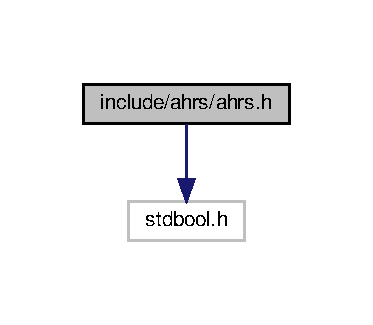
\includegraphics[width=179pt]{ahrs_8h__incl}
\end{center}
\end{figure}
\subsection*{Enumerations}
\begin{DoxyCompactItemize}
\item 
\mbox{\Hypertarget{ahrs_8h_a726ca809ffd3d67ab4b8476646f26635}\label{ahrs_8h_a726ca809ffd3d67ab4b8476646f26635}} 
enum \{ {\bfseries C\+O\+M\+P\+O\+N\+E\+N\+T\+\_\+\+M\+IN}, 
{\bfseries C\+O\+M\+P\+O\+N\+E\+N\+T\+\_\+\+M\+AX}
 \}
\item 
\mbox{\Hypertarget{ahrs_8h_a32d66f8d6f6a878b79f6a18c18fb85cf}\label{ahrs_8h_a32d66f8d6f6a878b79f6a18c18fb85cf}} 
enum {\bfseries att\+\_\+axis} \{ {\bfseries Y\+AW}, 
{\bfseries P\+I\+T\+CH}, 
{\bfseries R\+O\+LL}, 
{\bfseries N\+U\+M\+\_\+\+A\+T\+T\+\_\+\+A\+X\+ES}
 \}
\item 
\mbox{\Hypertarget{ahrs_8h_a98e4c2ebd3776f2226e168117904d6c1}\label{ahrs_8h_a98e4c2ebd3776f2226e168117904d6c1}} 
enum {\bfseries accel\+\_\+axis} \{ {\bfseries S\+W\+AY}, 
{\bfseries H\+E\+A\+VE}, 
{\bfseries S\+U\+R\+GE}, 
{\bfseries N\+U\+M\+\_\+\+A\+C\+C\+E\+L\+\_\+\+A\+X\+ES}
 \}
\end{DoxyCompactItemize}
\subsection*{Functions}
\begin{DoxyCompactItemize}
\item 
int \hyperlink{ahrs_8h_a653d935b0864f7e1ee7aa4dfbb522fcc}{ahrs\+\_\+cont\+\_\+start} ()
\begin{DoxyCompactList}\small\item\em Tells A\+H\+RS to start sending data in continous mode. \end{DoxyCompactList}\item 
float \hyperlink{ahrs_8h_a8432ad8e6e8fcc865fbb5d4e374b7c59}{ahrs\+\_\+att} (enum att\+\_\+axis dir)
\begin{DoxyCompactList}\small\item\em Tells A\+H\+RS to return angle for a certain direction. \end{DoxyCompactList}\item 
float \hyperlink{ahrs_8h_a49574e1c0ff13ef5edd5ea8d4d3d2914}{ahrs\+\_\+accel} (enum accel\+\_\+axis dir)
\begin{DoxyCompactList}\small\item\em Tells A\+H\+RS to return acceleration for certain direction. \end{DoxyCompactList}\item 
uint\+\_\+fast8\+\_\+t \hyperlink{ahrs_8h_aabcd9bcc5487394de174cb4b78f01d25}{ahrs\+\_\+headingstatus} ()
\begin{DoxyCompactList}\small\item\em Tells A\+H\+RS to return accuracy of current data. \end{DoxyCompactList}\item 
bool \hyperlink{ahrs_8h_a13682875d497e50e1b7bf5e5d173e154}{ahrs\+\_\+att\+\_\+update} ()
\begin{DoxyCompactList}\small\item\em Updates A\+H\+RS data. \end{DoxyCompactList}\item 
int \hyperlink{ahrs_8h_a9298af19f8651e14c0f43505c2196876}{ahrs\+\_\+att\+\_\+recv} ()
\begin{DoxyCompactList}\small\item\em Determines whether A\+H\+RS is returning data. \end{DoxyCompactList}\item 
void \hyperlink{ahrs_8h_a76fe8dc1638d7c89f7e14bc86238283c}{ahrs\+\_\+parse\+\_\+att\+\_\+reset} ()
\begin{DoxyCompactList}\small\item\em Discards incomplete A\+H\+RS data. \end{DoxyCompactList}\item 
\mbox{\Hypertarget{ahrs_8h_aa55ad38ec0330c9981d4d25742d1bb65}\label{ahrs_8h_aa55ad38ec0330c9981d4d25742d1bb65}} 
int {\bfseries ahrs\+\_\+set\+\_\+datacomp} ()
\end{DoxyCompactItemize}
\subsection*{Variables}
\begin{DoxyCompactItemize}
\item 
\mbox{\Hypertarget{ahrs_8h_a4f242cea3e7c041553bf2648729d6598}\label{ahrs_8h_a4f242cea3e7c041553bf2648729d6598}} 
float const {\bfseries ahrs\+\_\+range} \mbox{[}N\+U\+M\+\_\+\+A\+T\+T\+\_\+\+A\+X\+ES\mbox{]}\mbox{[}2\mbox{]}
\end{DoxyCompactItemize}


\subsection{Detailed Description}
Interface function definitions for the A\+H\+RS. 

\begin{DoxyAuthor}{Author}
Seth Girvan (Lord) 
\end{DoxyAuthor}


\subsection{Function Documentation}
\mbox{\Hypertarget{ahrs_8h_a49574e1c0ff13ef5edd5ea8d4d3d2914}\label{ahrs_8h_a49574e1c0ff13ef5edd5ea8d4d3d2914}} 
\index{ahrs.\+h@{ahrs.\+h}!ahrs\+\_\+accel@{ahrs\+\_\+accel}}
\index{ahrs\+\_\+accel@{ahrs\+\_\+accel}!ahrs.\+h@{ahrs.\+h}}
\subsubsection{\texorpdfstring{ahrs\+\_\+accel()}{ahrs\_accel()}}
{\footnotesize\ttfamily float ahrs\+\_\+accel (\begin{DoxyParamCaption}\item[{enum accel\+\_\+axis}]{dir }\end{DoxyParamCaption})}



Tells A\+H\+RS to return acceleration for certain direction. 

The coordinates are left-\/handed with positive heave up, positive sway left, and positive surge back.


\begin{DoxyParams}{Parameters}
{\em dir} & The wanted direction. \\
\hline
\end{DoxyParams}
\begin{DoxyReturn}{Returns}
The accelerometer value in G received from the ahrs for the dir. 
\end{DoxyReturn}
\mbox{\Hypertarget{ahrs_8h_a8432ad8e6e8fcc865fbb5d4e374b7c59}\label{ahrs_8h_a8432ad8e6e8fcc865fbb5d4e374b7c59}} 
\index{ahrs.\+h@{ahrs.\+h}!ahrs\+\_\+att@{ahrs\+\_\+att}}
\index{ahrs\+\_\+att@{ahrs\+\_\+att}!ahrs.\+h@{ahrs.\+h}}
\subsubsection{\texorpdfstring{ahrs\+\_\+att()}{ahrs\_att()}}
{\footnotesize\ttfamily float ahrs\+\_\+att (\begin{DoxyParamCaption}\item[{enum att\+\_\+axis}]{dir }\end{DoxyParamCaption})}



Tells A\+H\+RS to return angle for a certain direction. 

If the ahrs is in degrees mode the values will range per ahrs\+\_\+range\mbox{[}dir\mbox{]}.

The values returned will not changed until \hyperlink{ahrs_8h_a13682875d497e50e1b7bf5e5d173e154}{ahrs\+\_\+att\+\_\+update()} is called and it returns true.


\begin{DoxyParams}{Parameters}
{\em dir} & The wanted direction. \\
\hline
\end{DoxyParams}
\begin{DoxyReturn}{Returns}
The value received from the ahrs for the passed direction. 
\end{DoxyReturn}
\mbox{\Hypertarget{ahrs_8h_a9298af19f8651e14c0f43505c2196876}\label{ahrs_8h_a9298af19f8651e14c0f43505c2196876}} 
\index{ahrs.\+h@{ahrs.\+h}!ahrs\+\_\+att\+\_\+recv@{ahrs\+\_\+att\+\_\+recv}}
\index{ahrs\+\_\+att\+\_\+recv@{ahrs\+\_\+att\+\_\+recv}!ahrs.\+h@{ahrs.\+h}}
\subsubsection{\texorpdfstring{ahrs\+\_\+att\+\_\+recv()}{ahrs\_att\_recv()}}
{\footnotesize\ttfamily int ahrs\+\_\+att\+\_\+recv (\begin{DoxyParamCaption}{ }\end{DoxyParamCaption})}



Determines whether A\+H\+RS is returning data. 

\begin{DoxyReturn}{Returns}
True if at least one valid data set has been completely read from the ahrs. 
\end{DoxyReturn}
\mbox{\Hypertarget{ahrs_8h_a13682875d497e50e1b7bf5e5d173e154}\label{ahrs_8h_a13682875d497e50e1b7bf5e5d173e154}} 
\index{ahrs.\+h@{ahrs.\+h}!ahrs\+\_\+att\+\_\+update@{ahrs\+\_\+att\+\_\+update}}
\index{ahrs\+\_\+att\+\_\+update@{ahrs\+\_\+att\+\_\+update}!ahrs.\+h@{ahrs.\+h}}
\subsubsection{\texorpdfstring{ahrs\+\_\+att\+\_\+update()}{ahrs\_att\_update()}}
{\footnotesize\ttfamily bool ahrs\+\_\+att\+\_\+update (\begin{DoxyParamCaption}{ }\end{DoxyParamCaption})}



Updates A\+H\+RS data. 

Updates the values returned by ahrs\+\_\+att to the newest complete set of data that has been received from the ahrs before some point in time within this function\textquotesingle{}s lifetime.

Should only be called between complete \char`\"{}uses\char`\"{} of the attitude data to avoid using disparate data together (ie between runs of a \hyperlink{structPID}{P\+ID} routine).

\begin{DoxyReturn}{Returns}
True when there has been a new complete set of data received from the ahrs since the last time \hyperlink{ahrs_8h_a13682875d497e50e1b7bf5e5d173e154}{ahrs\+\_\+att\+\_\+update()} has been called. 
\end{DoxyReturn}
\mbox{\Hypertarget{ahrs_8h_a653d935b0864f7e1ee7aa4dfbb522fcc}\label{ahrs_8h_a653d935b0864f7e1ee7aa4dfbb522fcc}} 
\index{ahrs.\+h@{ahrs.\+h}!ahrs\+\_\+cont\+\_\+start@{ahrs\+\_\+cont\+\_\+start}}
\index{ahrs\+\_\+cont\+\_\+start@{ahrs\+\_\+cont\+\_\+start}!ahrs.\+h@{ahrs.\+h}}
\subsubsection{\texorpdfstring{ahrs\+\_\+cont\+\_\+start()}{ahrs\_cont\_start()}}
{\footnotesize\ttfamily int ahrs\+\_\+cont\+\_\+start (\begin{DoxyParamCaption}{ }\end{DoxyParamCaption})}



Tells A\+H\+RS to start sending data in continous mode. 

Make sure the desired data components are set first, such as with ahrs\+\_\+set\+\_\+datacomp().

\begin{DoxyReturn}{Returns}
0 on success 
\end{DoxyReturn}
\mbox{\Hypertarget{ahrs_8h_aabcd9bcc5487394de174cb4b78f01d25}\label{ahrs_8h_aabcd9bcc5487394de174cb4b78f01d25}} 
\index{ahrs.\+h@{ahrs.\+h}!ahrs\+\_\+headingstatus@{ahrs\+\_\+headingstatus}}
\index{ahrs\+\_\+headingstatus@{ahrs\+\_\+headingstatus}!ahrs.\+h@{ahrs.\+h}}
\subsubsection{\texorpdfstring{ahrs\+\_\+headingstatus()}{ahrs\_headingstatus()}}
{\footnotesize\ttfamily uint\+\_\+fast8\+\_\+t ahrs\+\_\+headingstatus (\begin{DoxyParamCaption}{ }\end{DoxyParamCaption})}



Tells A\+H\+RS to return accuracy of current data. 

Values\+: 1\+: uncertainty less than 2 degrees 2\+: uncertainty between 2 and 10 degres 3\+: uncertainty greater than 10 degrees However, it may give other values (I have known it to give the value 0).

\begin{DoxyReturn}{Returns}
The k\+Heading\+Status component from the ahrs associated with the current attitude data. 
\end{DoxyReturn}
\mbox{\Hypertarget{ahrs_8h_a76fe8dc1638d7c89f7e14bc86238283c}\label{ahrs_8h_a76fe8dc1638d7c89f7e14bc86238283c}} 
\index{ahrs.\+h@{ahrs.\+h}!ahrs\+\_\+parse\+\_\+att\+\_\+reset@{ahrs\+\_\+parse\+\_\+att\+\_\+reset}}
\index{ahrs\+\_\+parse\+\_\+att\+\_\+reset@{ahrs\+\_\+parse\+\_\+att\+\_\+reset}!ahrs.\+h@{ahrs.\+h}}
\subsubsection{\texorpdfstring{ahrs\+\_\+parse\+\_\+att\+\_\+reset()}{ahrs\_parse\_att\_reset()}}
{\footnotesize\ttfamily void ahrs\+\_\+parse\+\_\+att\+\_\+reset (\begin{DoxyParamCaption}{ }\end{DoxyParamCaption})}



Discards incomplete A\+H\+RS data. 

Causes any data from a current incomplete datagram to be discarded. The next received byte will be treated as potentially the start of a datagram.

Can be used due for, eg, a serial timeout for intra-\/datagram data. 
\hypertarget{crc__xmodem_8h}{}\section{include/ahrs/crc\+\_\+xmodem.h File Reference}
\label{crc__xmodem_8h}\index{include/ahrs/crc\+\_\+xmodem.\+h@{include/ahrs/crc\+\_\+xmodem.\+h}}


Helper macros for C\+R\+C-\/\+X\+M\+O\+D\+EM updating.  


{\ttfamily \#include \char`\"{}crc\+\_\+xmodem\+\_\+generic.\+h\char`\"{}}\newline
Include dependency graph for crc\+\_\+xmodem.\+h\+:
\nopagebreak
\begin{figure}[H]
\begin{center}
\leavevmode
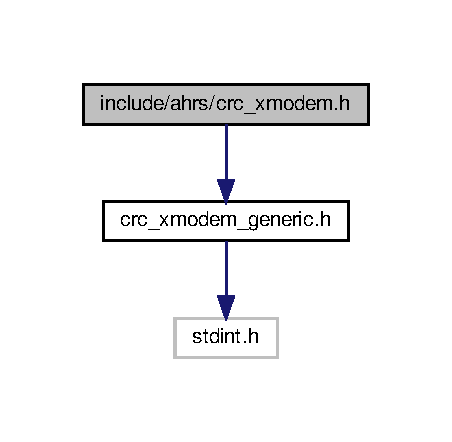
\includegraphics[width=217pt]{crc__xmodem_8h__incl}
\end{center}
\end{figure}
\subsection*{Macros}
\begin{DoxyCompactItemize}
\item 
\mbox{\Hypertarget{crc__xmodem_8h_abb06933ed9907921f240b9d301855d25}\label{crc__xmodem_8h_abb06933ed9907921f240b9d301855d25}} 
\#define {\bfseries C\+R\+C\+\_\+\+X\+M\+O\+D\+E\+M\+\_\+\+I\+N\+I\+T\+\_\+\+V\+AL}~0x0000U
\item 
\mbox{\Hypertarget{crc__xmodem_8h_a12fd495ff0805ef2335ae91a5de4a94e}\label{crc__xmodem_8h_a12fd495ff0805ef2335ae91a5de4a94e}} 
\#define {\bfseries crc\+\_\+xmodem\+\_\+update}(a,  b)~\hyperlink{crc__xmodem__generic_8h_a618a4e92162fc58fd2f3b8ba0b452e67}{generic\+\_\+crc\+\_\+xmodem\+\_\+update}(a, b)
\end{DoxyCompactItemize}


\subsection{Detailed Description}
Helper macros for C\+R\+C-\/\+X\+M\+O\+D\+EM updating. 

\begin{DoxyAuthor}{Author}
Seth Girvan (Lord) 
\end{DoxyAuthor}

\hypertarget{crc__xmodem__generic_8h}{}\section{include/ahrs/crc\+\_\+xmodem\+\_\+generic.h File Reference}
\label{crc__xmodem__generic_8h}\index{include/ahrs/crc\+\_\+xmodem\+\_\+generic.\+h@{include/ahrs/crc\+\_\+xmodem\+\_\+generic.\+h}}


C\+RC update functions for testing.  


{\ttfamily \#include $<$stdint.\+h$>$}\newline
Include dependency graph for crc\+\_\+xmodem\+\_\+generic.\+h\+:\nopagebreak
\begin{figure}[H]
\begin{center}
\leavevmode
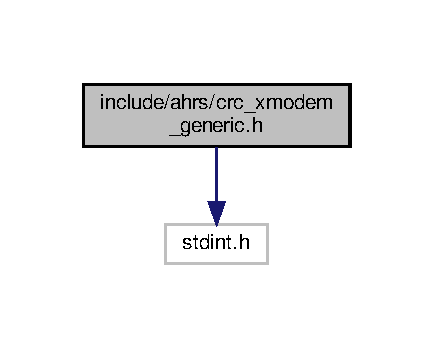
\includegraphics[width=208pt]{crc__xmodem__generic_8h__incl}
\end{center}
\end{figure}
This graph shows which files directly or indirectly include this file\+:\nopagebreak
\begin{figure}[H]
\begin{center}
\leavevmode
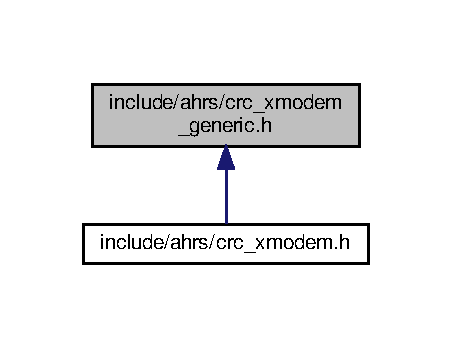
\includegraphics[width=217pt]{crc__xmodem__generic_8h__dep__incl}
\end{center}
\end{figure}
\subsection*{Functions}
\begin{DoxyCompactItemize}
\item 
uint16\+\_\+t \hyperlink{crc__xmodem__generic_8h_a618a4e92162fc58fd2f3b8ba0b452e67}{generic\+\_\+crc\+\_\+xmodem\+\_\+update} (uint16\+\_\+t crc, uint8\+\_\+t data)
\begin{DoxyCompactList}\small\item\em Update a C\+RC with 8 bits of additional data. \end{DoxyCompactList}\end{DoxyCompactItemize}


\subsection{Detailed Description}
C\+RC update functions for testing. 

\begin{DoxyAuthor}{Author}
Seth Girvan (Lord) 
\end{DoxyAuthor}


\subsection{Function Documentation}
\mbox{\Hypertarget{crc__xmodem__generic_8h_a618a4e92162fc58fd2f3b8ba0b452e67}\label{crc__xmodem__generic_8h_a618a4e92162fc58fd2f3b8ba0b452e67}} 
\index{crc\+\_\+xmodem\+\_\+generic.\+h@{crc\+\_\+xmodem\+\_\+generic.\+h}!generic\+\_\+crc\+\_\+xmodem\+\_\+update@{generic\+\_\+crc\+\_\+xmodem\+\_\+update}}
\index{generic\+\_\+crc\+\_\+xmodem\+\_\+update@{generic\+\_\+crc\+\_\+xmodem\+\_\+update}!crc\+\_\+xmodem\+\_\+generic.\+h@{crc\+\_\+xmodem\+\_\+generic.\+h}}
\subsubsection{\texorpdfstring{generic\+\_\+crc\+\_\+xmodem\+\_\+update()}{generic\_crc\_xmodem\_update()}}
{\footnotesize\ttfamily uint16\+\_\+t generic\+\_\+crc\+\_\+xmodem\+\_\+update (\begin{DoxyParamCaption}\item[{uint16\+\_\+t}]{crc,  }\item[{uint8\+\_\+t}]{data }\end{DoxyParamCaption})}



Update a C\+RC with 8 bits of additional data. 

This is unoptimized and meant to be used for testing on computer. On avr, one should use the optimized \+\_\+crc\+\_\+xmodem\+\_\+update() in util/crc16.\+h

\begin{DoxyReturn}{Returns}
New C\+RC. 
\end{DoxyReturn}

\hypertarget{io__ahrs_8h}{}\section{include/ahrs/io\+\_\+ahrs.h File Reference}
\label{io__ahrs_8h}\index{include/ahrs/io\+\_\+ahrs.\+h@{include/ahrs/io\+\_\+ahrs.\+h}}


Low-\/level communication functions for A\+H\+RS.  


{\ttfamily \#include $<$stdio.\+h$>$}\newline
{\ttfamily \#include $<$stdbool.\+h$>$}\newline
Include dependency graph for io\+\_\+ahrs.\+h\+:
\nopagebreak
\begin{figure}[H]
\begin{center}
\leavevmode
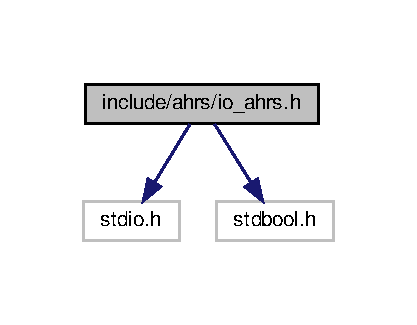
\includegraphics[width=200pt]{io__ahrs_8h__incl}
\end{center}
\end{figure}
\subsection*{Functions}
\begin{DoxyCompactItemize}
\item 
void \hyperlink{io__ahrs_8h_a312fc51f6c9726e41cfbc780cfcfecdc}{io\+\_\+ahrs\+\_\+init} (char const $\ast$path)
\begin{DoxyCompactList}\small\item\em Prepare A\+H\+RS to receive data. \end{DoxyCompactList}\item 
void \hyperlink{io__ahrs_8h_a9db69393e769bcdd5ddc9ec5f125d11d}{io\+\_\+ahrs\+\_\+clean} ()
\begin{DoxyCompactList}\small\item\em Disable A\+H\+RS transmit and receive. \end{DoxyCompactList}\item 
int \hyperlink{io__ahrs_8h_afa79bf757710a1cad094f1e15eb634b7}{io\+\_\+ahrs\+\_\+recv\+\_\+start} (int($\ast$handler)())
\begin{DoxyCompactList}\small\item\em Tells A\+H\+RS to start receiving attitude data. \end{DoxyCompactList}\item 
void \hyperlink{io__ahrs_8h_a2ee2459ddd2dca694bef3e6fb9b1cd54}{io\+\_\+ahrs\+\_\+recv\+\_\+stop} ()
\begin{DoxyCompactList}\small\item\em Tells A\+H\+RS to start receiving attitude data. \end{DoxyCompactList}\item 
bool \hyperlink{io__ahrs_8h_a7b33a09e7c9290bcdeebf2602a54ee3d}{io\+\_\+ahrs\+\_\+tripbuf\+\_\+update} ()
\item 
void \hyperlink{io__ahrs_8h_ac133fdc94162c623c5325f907ade9e4a}{io\+\_\+ahrs\+\_\+tripbuf\+\_\+offer} ()
\item 
unsigned char \hyperlink{io__ahrs_8h_a7e158c735ff3b4a8b84cd5bd552c4954}{io\+\_\+ahrs\+\_\+tripbuf\+\_\+read} ()
\item 
unsigned char \hyperlink{io__ahrs_8h_a7690920caf5d41a90442ca049336778c}{io\+\_\+ahrs\+\_\+tripbuf\+\_\+write} ()
\end{DoxyCompactItemize}
\subsection*{Variables}
\begin{DoxyCompactItemize}
\item 
F\+I\+LE $\ast$ \hyperlink{io__ahrs_8h_a7c946296e6bffe77d1c08cdcbd4def85}{io\+\_\+ahrs}
\end{DoxyCompactItemize}


\subsection{Detailed Description}
Low-\/level communication functions for A\+H\+RS. 

\begin{DoxyAuthor}{Author}
Seth Girvan (Lord) 
\end{DoxyAuthor}


\subsection{Function Documentation}
\mbox{\Hypertarget{io__ahrs_8h_a9db69393e769bcdd5ddc9ec5f125d11d}\label{io__ahrs_8h_a9db69393e769bcdd5ddc9ec5f125d11d}} 
\index{io\+\_\+ahrs.\+h@{io\+\_\+ahrs.\+h}!io\+\_\+ahrs\+\_\+clean@{io\+\_\+ahrs\+\_\+clean}}
\index{io\+\_\+ahrs\+\_\+clean@{io\+\_\+ahrs\+\_\+clean}!io\+\_\+ahrs.\+h@{io\+\_\+ahrs.\+h}}
\subsubsection{\texorpdfstring{io\+\_\+ahrs\+\_\+clean()}{io\_ahrs\_clean()}}
{\footnotesize\ttfamily void io\+\_\+ahrs\+\_\+clean (\begin{DoxyParamCaption}{ }\end{DoxyParamCaption})}



Disable A\+H\+RS transmit and receive. 

Unimplemented.

\begin{DoxyReturn}{Returns}
Void. 
\end{DoxyReturn}
\mbox{\Hypertarget{io__ahrs_8h_a312fc51f6c9726e41cfbc780cfcfecdc}\label{io__ahrs_8h_a312fc51f6c9726e41cfbc780cfcfecdc}} 
\index{io\+\_\+ahrs.\+h@{io\+\_\+ahrs.\+h}!io\+\_\+ahrs\+\_\+init@{io\+\_\+ahrs\+\_\+init}}
\index{io\+\_\+ahrs\+\_\+init@{io\+\_\+ahrs\+\_\+init}!io\+\_\+ahrs.\+h@{io\+\_\+ahrs.\+h}}
\subsubsection{\texorpdfstring{io\+\_\+ahrs\+\_\+init()}{io\_ahrs\_init()}}
{\footnotesize\ttfamily void io\+\_\+ahrs\+\_\+init (\begin{DoxyParamCaption}\item[{char const $\ast$}]{path }\end{DoxyParamCaption})}



Prepare A\+H\+RS to receive data. 

Assumes uart N\+U\+S\+A\+RT will be used and connected with the ahrs I\+E\+A-\/232 interface via a ttl$<$-\/$>$I\+E\+A-\/232 converter.

Per the T\+R\+AX P\+NI user manual\+: Start Bits\+: 1 Number of Data Bits\+: 8 Stop Bits\+: 1 Parity\+: none Baud\+: B\+A\+UD


\begin{DoxyParams}{Parameters}
{\em path} & Path to A\+H\+RS from main computer, unused at the moment. \\
\hline
\end{DoxyParams}
\begin{DoxyReturn}{Returns}
Void. 
\end{DoxyReturn}
\mbox{\Hypertarget{io__ahrs_8h_afa79bf757710a1cad094f1e15eb634b7}\label{io__ahrs_8h_afa79bf757710a1cad094f1e15eb634b7}} 
\index{io\+\_\+ahrs.\+h@{io\+\_\+ahrs.\+h}!io\+\_\+ahrs\+\_\+recv\+\_\+start@{io\+\_\+ahrs\+\_\+recv\+\_\+start}}
\index{io\+\_\+ahrs\+\_\+recv\+\_\+start@{io\+\_\+ahrs\+\_\+recv\+\_\+start}!io\+\_\+ahrs.\+h@{io\+\_\+ahrs.\+h}}
\subsubsection{\texorpdfstring{io\+\_\+ahrs\+\_\+recv\+\_\+start()}{io\_ahrs\_recv\_start()}}
{\footnotesize\ttfamily int io\+\_\+ahrs\+\_\+recv\+\_\+start (\begin{DoxyParamCaption}\item[{int($\ast$)()}]{handler }\end{DoxyParamCaption})}



Tells A\+H\+RS to start receiving attitude data. 

\begin{DoxyReturn}{Returns}
0 on success 
\end{DoxyReturn}
\mbox{\Hypertarget{io__ahrs_8h_a2ee2459ddd2dca694bef3e6fb9b1cd54}\label{io__ahrs_8h_a2ee2459ddd2dca694bef3e6fb9b1cd54}} 
\index{io\+\_\+ahrs.\+h@{io\+\_\+ahrs.\+h}!io\+\_\+ahrs\+\_\+recv\+\_\+stop@{io\+\_\+ahrs\+\_\+recv\+\_\+stop}}
\index{io\+\_\+ahrs\+\_\+recv\+\_\+stop@{io\+\_\+ahrs\+\_\+recv\+\_\+stop}!io\+\_\+ahrs.\+h@{io\+\_\+ahrs.\+h}}
\subsubsection{\texorpdfstring{io\+\_\+ahrs\+\_\+recv\+\_\+stop()}{io\_ahrs\_recv\_stop()}}
{\footnotesize\ttfamily void io\+\_\+ahrs\+\_\+recv\+\_\+stop (\begin{DoxyParamCaption}{ }\end{DoxyParamCaption})}



Tells A\+H\+RS to start receiving attitude data. 

\begin{DoxyReturn}{Returns}
0 on success 
\end{DoxyReturn}
\mbox{\Hypertarget{io__ahrs_8h_ac133fdc94162c623c5325f907ade9e4a}\label{io__ahrs_8h_ac133fdc94162c623c5325f907ade9e4a}} 
\index{io\+\_\+ahrs.\+h@{io\+\_\+ahrs.\+h}!io\+\_\+ahrs\+\_\+tripbuf\+\_\+offer@{io\+\_\+ahrs\+\_\+tripbuf\+\_\+offer}}
\index{io\+\_\+ahrs\+\_\+tripbuf\+\_\+offer@{io\+\_\+ahrs\+\_\+tripbuf\+\_\+offer}!io\+\_\+ahrs.\+h@{io\+\_\+ahrs.\+h}}
\subsubsection{\texorpdfstring{io\+\_\+ahrs\+\_\+tripbuf\+\_\+offer()}{io\_ahrs\_tripbuf\_offer()}}
{\footnotesize\ttfamily void io\+\_\+ahrs\+\_\+tripbuf\+\_\+offer (\begin{DoxyParamCaption}{ }\end{DoxyParamCaption})}

Makes the current write index available to io\+\_\+ahrs\+\_\+tripbuf\+\_\+update, and changes the value returned by io\+\_\+ahrs\+\_\+tripbuf\+\_\+write.

May interrupt io\+\_\+ahrs\+\_\+tripbuf\+\_\+update, but may not be interrupted by it \mbox{\Hypertarget{io__ahrs_8h_a7e158c735ff3b4a8b84cd5bd552c4954}\label{io__ahrs_8h_a7e158c735ff3b4a8b84cd5bd552c4954}} 
\index{io\+\_\+ahrs.\+h@{io\+\_\+ahrs.\+h}!io\+\_\+ahrs\+\_\+tripbuf\+\_\+read@{io\+\_\+ahrs\+\_\+tripbuf\+\_\+read}}
\index{io\+\_\+ahrs\+\_\+tripbuf\+\_\+read@{io\+\_\+ahrs\+\_\+tripbuf\+\_\+read}!io\+\_\+ahrs.\+h@{io\+\_\+ahrs.\+h}}
\subsubsection{\texorpdfstring{io\+\_\+ahrs\+\_\+tripbuf\+\_\+read()}{io\_ahrs\_tripbuf\_read()}}
{\footnotesize\ttfamily unsigned char io\+\_\+ahrs\+\_\+tripbuf\+\_\+read (\begin{DoxyParamCaption}{ }\end{DoxyParamCaption})}

returns the index of the buffer the data consumer should read from. Only changes if io\+\_\+ahrs\+\_\+tripbuf\+\_\+update is called and returns true. \mbox{\Hypertarget{io__ahrs_8h_a7b33a09e7c9290bcdeebf2602a54ee3d}\label{io__ahrs_8h_a7b33a09e7c9290bcdeebf2602a54ee3d}} 
\index{io\+\_\+ahrs.\+h@{io\+\_\+ahrs.\+h}!io\+\_\+ahrs\+\_\+tripbuf\+\_\+update@{io\+\_\+ahrs\+\_\+tripbuf\+\_\+update}}
\index{io\+\_\+ahrs\+\_\+tripbuf\+\_\+update@{io\+\_\+ahrs\+\_\+tripbuf\+\_\+update}!io\+\_\+ahrs.\+h@{io\+\_\+ahrs.\+h}}
\subsubsection{\texorpdfstring{io\+\_\+ahrs\+\_\+tripbuf\+\_\+update()}{io\_ahrs\_tripbuf\_update()}}
{\footnotesize\ttfamily bool io\+\_\+ahrs\+\_\+tripbuf\+\_\+update (\begin{DoxyParamCaption}{ }\end{DoxyParamCaption})}

Causes io\+\_\+ahrs\+\_\+tripbuf\+\_\+read to return index that was most recently \textquotesingle{}submitted\textquotesingle{} by io\+\_\+ahrs\+\_\+tripbuf\+\_\+offer.

This should only be run between complete \textquotesingle{}uses\textquotesingle{} of the data, to avoid using disparate data.

Unfortunately, since there is no way to have a lock-\/free/interruptable triple buffer implementation on the avr, this has to be platform-\/specific. A lock-\/free ring buffer would not handle cases when the producer is faster than the consumer well.

May be interrupted by io\+\_\+ahrs\+\_\+tripbuf\+\_\+offer, but cannot interrupt it (ie this can be interrupted by handler\+\_\+ahrs\+\_\+recv, but one probably does not want to call it from handler\+\_\+ahrs\+\_\+recv).

returns whether there has been any new data since last call \mbox{\Hypertarget{io__ahrs_8h_a7690920caf5d41a90442ca049336778c}\label{io__ahrs_8h_a7690920caf5d41a90442ca049336778c}} 
\index{io\+\_\+ahrs.\+h@{io\+\_\+ahrs.\+h}!io\+\_\+ahrs\+\_\+tripbuf\+\_\+write@{io\+\_\+ahrs\+\_\+tripbuf\+\_\+write}}
\index{io\+\_\+ahrs\+\_\+tripbuf\+\_\+write@{io\+\_\+ahrs\+\_\+tripbuf\+\_\+write}!io\+\_\+ahrs.\+h@{io\+\_\+ahrs.\+h}}
\subsubsection{\texorpdfstring{io\+\_\+ahrs\+\_\+tripbuf\+\_\+write()}{io\_ahrs\_tripbuf\_write()}}
{\footnotesize\ttfamily unsigned char io\+\_\+ahrs\+\_\+tripbuf\+\_\+write (\begin{DoxyParamCaption}{ }\end{DoxyParamCaption})}

returns the index of the buffer the data producer should write to. Only changes when io\+\_\+ahrs\+\_\+tripbuf\+\_\+offer is called. 

\subsection{Variable Documentation}
\mbox{\Hypertarget{io__ahrs_8h_a7c946296e6bffe77d1c08cdcbd4def85}\label{io__ahrs_8h_a7c946296e6bffe77d1c08cdcbd4def85}} 
\index{io\+\_\+ahrs.\+h@{io\+\_\+ahrs.\+h}!io\+\_\+ahrs@{io\+\_\+ahrs}}
\index{io\+\_\+ahrs@{io\+\_\+ahrs}!io\+\_\+ahrs.\+h@{io\+\_\+ahrs.\+h}}
\subsubsection{\texorpdfstring{io\+\_\+ahrs}{io\_ahrs}}
{\footnotesize\ttfamily F\+I\+LE$\ast$ io\+\_\+ahrs}

io with this is blocking, so one might use normal stdio functions directly on it when they are willing to wait, eg sending initial configuration data, but to be able to handle asynchronous io, one should use io\+\_\+ahrs\+\_\+...\+\_\+start, which allows us to process data on the fly and avoid polling. 
\hypertarget{dvl_8h}{}\section{include/dvl/dvl.h File Reference}
\label{dvl_8h}\index{include/dvl/dvl.\+h@{include/dvl/dvl.\+h}}


Interface function definitions for D\+VL.  


{\ttfamily \#include $<$stdbool.\+h$>$}\newline
Include dependency graph for dvl.\+h\+:\nopagebreak
\begin{figure}[H]
\begin{center}
\leavevmode
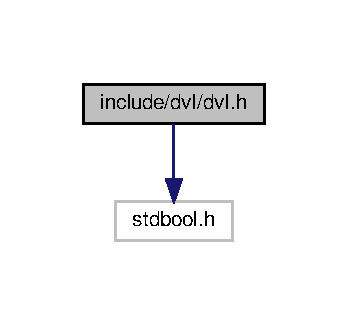
\includegraphics[width=167pt]{dvl_8h__incl}
\end{center}
\end{figure}
\subsection*{Functions}
\begin{DoxyCompactItemize}
\item 
\mbox{\Hypertarget{dvl_8h_ace13fbd095b6f793b7704a717902cef2}\label{dvl_8h_ace13fbd095b6f793b7704a717902cef2}} 
void \hyperlink{dvl_8h_ace13fbd095b6f793b7704a717902cef2}{dvl\+\_\+set\+\_\+data\+\_\+format} ()
\begin{DoxyCompactList}\small\item\em Configures proper D\+VL data components. \end{DoxyCompactList}\item 
\mbox{\Hypertarget{dvl_8h_a88885ad4d9407ea44a0d1473c85e459b}\label{dvl_8h_a88885ad4d9407ea44a0d1473c85e459b}} 
void \hyperlink{dvl_8h_a88885ad4d9407ea44a0d1473c85e459b}{dvl\+\_\+begin\+\_\+pinging} ()
\begin{DoxyCompactList}\small\item\em Tells D\+VL to begin pinging. \end{DoxyCompactList}\item 
\mbox{\Hypertarget{dvl_8h_a3e2d1045f92e30c7f8e21d2c54af5d8d}\label{dvl_8h_a3e2d1045f92e30c7f8e21d2c54af5d8d}} 
void \hyperlink{dvl_8h_a3e2d1045f92e30c7f8e21d2c54af5d8d}{reset\+\_\+parser} ()
\begin{DoxyCompactList}\small\item\em Discards the datagram that is being parsed. \end{DoxyCompactList}\item 
bool \hyperlink{dvl_8h_acd282756a658fc5e2fe729d9684263d1}{dvl\+\_\+data\+\_\+update} ()
\begin{DoxyCompactList}\small\item\em Replaces old data on the D\+VL with new data. \end{DoxyCompactList}\item 
int32\+\_\+t \hyperlink{dvl_8h_a42627cfa581f9b51ed01025e5deaf16e}{dvl\+\_\+get\+\_\+starboard\+\_\+vel} ()
\begin{DoxyCompactList}\small\item\em Finds velocity over bottom towards starboard. \end{DoxyCompactList}\item 
int32\+\_\+t \hyperlink{dvl_8h_a836f3040e47b915729718c2cdd6a9064}{dvl\+\_\+get\+\_\+forward\+\_\+vel} ()
\begin{DoxyCompactList}\small\item\em Finds velocity over bottom towards bow. \end{DoxyCompactList}\item 
int32\+\_\+t \hyperlink{dvl_8h_a5e5bdfedb1dcd23f982911e43552dea0}{dvl\+\_\+get\+\_\+upward\+\_\+vel} ()
\begin{DoxyCompactList}\small\item\em Finds velocity over bottom towards surface. \end{DoxyCompactList}\item 
int32\+\_\+t \hyperlink{dvl_8h_a67d1828f6fe430d9e886609d6c258f10}{dvl\+\_\+get\+\_\+range\+\_\+to\+\_\+bottom} ()
\begin{DoxyCompactList}\small\item\em Finds distance to bottom. \end{DoxyCompactList}\item 
bool \hyperlink{dvl_8h_ae35718ff4c189bdaaf55edc0288ad7fe}{dvl\+\_\+receive\+\_\+handler} ()
\begin{DoxyCompactList}\small\item\em Parses and processes received data. \end{DoxyCompactList}\item 
int \hyperlink{dvl_8h_aee5f5ff835ae272fd7d1e1fb9bf347fb}{send\+\_\+command} (char $\ast$cmd, bool wait)
\begin{DoxyCompactList}\small\item\em Sends command for D\+VL to process. \end{DoxyCompactList}\end{DoxyCompactItemize}


\subsection{Detailed Description}
Interface function definitions for D\+VL. 

\begin{DoxyAuthor}{Author}
Timothy Kanarsky 

David Zhang 
\end{DoxyAuthor}


\subsection{Function Documentation}
\mbox{\Hypertarget{dvl_8h_acd282756a658fc5e2fe729d9684263d1}\label{dvl_8h_acd282756a658fc5e2fe729d9684263d1}} 
\index{dvl.\+h@{dvl.\+h}!dvl\+\_\+data\+\_\+update@{dvl\+\_\+data\+\_\+update}}
\index{dvl\+\_\+data\+\_\+update@{dvl\+\_\+data\+\_\+update}!dvl.\+h@{dvl.\+h}}
\subsubsection{\texorpdfstring{dvl\+\_\+data\+\_\+update()}{dvl\_data\_update()}}
{\footnotesize\ttfamily bool dvl\+\_\+data\+\_\+update (\begin{DoxyParamCaption}{ }\end{DoxyParamCaption})}



Replaces old data on the D\+VL with new data. 

\begin{DoxyReturn}{Returns}
True on success. 
\end{DoxyReturn}
\mbox{\Hypertarget{dvl_8h_a836f3040e47b915729718c2cdd6a9064}\label{dvl_8h_a836f3040e47b915729718c2cdd6a9064}} 
\index{dvl.\+h@{dvl.\+h}!dvl\+\_\+get\+\_\+forward\+\_\+vel@{dvl\+\_\+get\+\_\+forward\+\_\+vel}}
\index{dvl\+\_\+get\+\_\+forward\+\_\+vel@{dvl\+\_\+get\+\_\+forward\+\_\+vel}!dvl.\+h@{dvl.\+h}}
\subsubsection{\texorpdfstring{dvl\+\_\+get\+\_\+forward\+\_\+vel()}{dvl\_get\_forward\_vel()}}
{\footnotesize\ttfamily int32\+\_\+t dvl\+\_\+get\+\_\+forward\+\_\+vel (\begin{DoxyParamCaption}{ }\end{DoxyParamCaption})}



Finds velocity over bottom towards bow. 

\begin{DoxyReturn}{Returns}
Velocity as 32-\/bit integer in 1um/s. 
\end{DoxyReturn}
\mbox{\Hypertarget{dvl_8h_a67d1828f6fe430d9e886609d6c258f10}\label{dvl_8h_a67d1828f6fe430d9e886609d6c258f10}} 
\index{dvl.\+h@{dvl.\+h}!dvl\+\_\+get\+\_\+range\+\_\+to\+\_\+bottom@{dvl\+\_\+get\+\_\+range\+\_\+to\+\_\+bottom}}
\index{dvl\+\_\+get\+\_\+range\+\_\+to\+\_\+bottom@{dvl\+\_\+get\+\_\+range\+\_\+to\+\_\+bottom}!dvl.\+h@{dvl.\+h}}
\subsubsection{\texorpdfstring{dvl\+\_\+get\+\_\+range\+\_\+to\+\_\+bottom()}{dvl\_get\_range\_to\_bottom()}}
{\footnotesize\ttfamily int32\+\_\+t dvl\+\_\+get\+\_\+range\+\_\+to\+\_\+bottom (\begin{DoxyParamCaption}{ }\end{DoxyParamCaption})}



Finds distance to bottom. 

Should not be negative. (\+:P)

\begin{DoxyReturn}{Returns}
Distance as 32-\/bit integer in 0.\+1mm. 
\end{DoxyReturn}
\mbox{\Hypertarget{dvl_8h_a42627cfa581f9b51ed01025e5deaf16e}\label{dvl_8h_a42627cfa581f9b51ed01025e5deaf16e}} 
\index{dvl.\+h@{dvl.\+h}!dvl\+\_\+get\+\_\+starboard\+\_\+vel@{dvl\+\_\+get\+\_\+starboard\+\_\+vel}}
\index{dvl\+\_\+get\+\_\+starboard\+\_\+vel@{dvl\+\_\+get\+\_\+starboard\+\_\+vel}!dvl.\+h@{dvl.\+h}}
\subsubsection{\texorpdfstring{dvl\+\_\+get\+\_\+starboard\+\_\+vel()}{dvl\_get\_starboard\_vel()}}
{\footnotesize\ttfamily int32\+\_\+t dvl\+\_\+get\+\_\+starboard\+\_\+vel (\begin{DoxyParamCaption}{ }\end{DoxyParamCaption})}



Finds velocity over bottom towards starboard. 

\begin{DoxyReturn}{Returns}
Velocity as 32-\/bit integer in 1um/s. 
\end{DoxyReturn}
\mbox{\Hypertarget{dvl_8h_a5e5bdfedb1dcd23f982911e43552dea0}\label{dvl_8h_a5e5bdfedb1dcd23f982911e43552dea0}} 
\index{dvl.\+h@{dvl.\+h}!dvl\+\_\+get\+\_\+upward\+\_\+vel@{dvl\+\_\+get\+\_\+upward\+\_\+vel}}
\index{dvl\+\_\+get\+\_\+upward\+\_\+vel@{dvl\+\_\+get\+\_\+upward\+\_\+vel}!dvl.\+h@{dvl.\+h}}
\subsubsection{\texorpdfstring{dvl\+\_\+get\+\_\+upward\+\_\+vel()}{dvl\_get\_upward\_vel()}}
{\footnotesize\ttfamily int32\+\_\+t dvl\+\_\+get\+\_\+upward\+\_\+vel (\begin{DoxyParamCaption}{ }\end{DoxyParamCaption})}



Finds velocity over bottom towards surface. 

\begin{DoxyReturn}{Returns}
Velocity as 32-\/bit integer in 1um/s. 
\end{DoxyReturn}
\mbox{\Hypertarget{dvl_8h_ae35718ff4c189bdaaf55edc0288ad7fe}\label{dvl_8h_ae35718ff4c189bdaaf55edc0288ad7fe}} 
\index{dvl.\+h@{dvl.\+h}!dvl\+\_\+receive\+\_\+handler@{dvl\+\_\+receive\+\_\+handler}}
\index{dvl\+\_\+receive\+\_\+handler@{dvl\+\_\+receive\+\_\+handler}!dvl.\+h@{dvl.\+h}}
\subsubsection{\texorpdfstring{dvl\+\_\+receive\+\_\+handler()}{dvl\_receive\_handler()}}
{\footnotesize\ttfamily bool dvl\+\_\+receive\+\_\+handler (\begin{DoxyParamCaption}{ }\end{DoxyParamCaption})}



Parses and processes received data. 

\begin{DoxyReturn}{Returns}
True when a complete datagram has been parsed. 
\end{DoxyReturn}
\mbox{\Hypertarget{dvl_8h_aee5f5ff835ae272fd7d1e1fb9bf347fb}\label{dvl_8h_aee5f5ff835ae272fd7d1e1fb9bf347fb}} 
\index{dvl.\+h@{dvl.\+h}!send\+\_\+command@{send\+\_\+command}}
\index{send\+\_\+command@{send\+\_\+command}!dvl.\+h@{dvl.\+h}}
\subsubsection{\texorpdfstring{send\+\_\+command()}{send\_command()}}
{\footnotesize\ttfamily int send\+\_\+command (\begin{DoxyParamCaption}\item[{char $\ast$}]{cmd,  }\item[{bool}]{wait }\end{DoxyParamCaption})}



Sends command for D\+VL to process. 


\begin{DoxyParams}{Parameters}
{\em cmd} & The command as a character. \\
\hline
{\em wait} & If true, waits until D\+VL is finished processing before sending the command. \\
\hline
\end{DoxyParams}
\begin{DoxyReturn}{Returns}
1 on success, negative number on error. 
\end{DoxyReturn}

\hypertarget{dvl__commands_8h}{}\section{include/dvl/dvl\+\_\+commands.h File Reference}
\label{dvl__commands_8h}\index{include/dvl/dvl\+\_\+commands.\+h@{include/dvl/dvl\+\_\+commands.\+h}}


Interface function definitions for D\+VL.  


\subsection*{Macros}
\begin{DoxyCompactItemize}
\item 
\mbox{\Hypertarget{dvl__commands_8h_adef3034178d2e2de064a8709350e8f01}\label{dvl__commands_8h_adef3034178d2e2de064a8709350e8f01}} 
\#define {\bfseries N\+U\+M\+\_\+\+C\+O\+M\+M\+A\+N\+DS}~12
\end{DoxyCompactItemize}
\subsection*{Variables}
\begin{DoxyCompactItemize}
\item 
\mbox{\Hypertarget{dvl__commands_8h_a8fc19b86e102436b966cc32b5748ae72}\label{dvl__commands_8h_a8fc19b86e102436b966cc32b5748ae72}} 
char $\ast$ {\bfseries break\+\_\+command} = \char`\"{}===\char`\"{}
\item 
char $\ast$ \hyperlink{dvl__commands_8h_a4005b50caf69d0e6e2eb922578ef2850}{setup\+\_\+commands} \mbox{[}N\+U\+M\+\_\+\+C\+O\+M\+M\+A\+N\+DS\mbox{]}
\begin{DoxyCompactList}\small\item\em Important setup commands. \end{DoxyCompactList}\item 
\mbox{\Hypertarget{dvl__commands_8h_a727a7a096d28f9baa4605f2060612184}\label{dvl__commands_8h_a727a7a096d28f9baa4605f2060612184}} 
char $\ast$ {\bfseries ping\+\_\+command} = \char`\"{}cs\textbackslash{}r\char`\"{}
\end{DoxyCompactItemize}


\subsection{Detailed Description}
Interface function definitions for D\+VL. 

\begin{DoxyAuthor}{Author}
Timothy Kanarsky 
\end{DoxyAuthor}


\subsection{Variable Documentation}
\mbox{\Hypertarget{dvl__commands_8h_a4005b50caf69d0e6e2eb922578ef2850}\label{dvl__commands_8h_a4005b50caf69d0e6e2eb922578ef2850}} 
\index{dvl\+\_\+commands.\+h@{dvl\+\_\+commands.\+h}!setup\+\_\+commands@{setup\+\_\+commands}}
\index{setup\+\_\+commands@{setup\+\_\+commands}!dvl\+\_\+commands.\+h@{dvl\+\_\+commands.\+h}}
\subsubsection{\texorpdfstring{setup\+\_\+commands}{setup\_commands}}
{\footnotesize\ttfamily char$\ast$ setup\+\_\+commands\mbox{[}N\+U\+M\+\_\+\+C\+O\+M\+M\+A\+N\+DS\mbox{]}}

{\bfseries Initial value\+:}
\begin{DoxyCode}
= \{
    \textcolor{stringliteral}{"CR1\(\backslash\)r"}, 
    \textcolor{stringliteral}{"BX00100\(\backslash\)r"}, 
    \textcolor{stringliteral}{"#BJ000110000\(\backslash\)r"}, 
    \textcolor{stringliteral}{"CF11110\(\backslash\)r"}, 
    
    \textcolor{stringliteral}{"EA-04500\(\backslash\)r"}, 
    \textcolor{stringliteral}{"ED00010\(\backslash\)r"}, 



    \textcolor{stringliteral}{"ES00\(\backslash\)r"},

    \textcolor{stringliteral}{"EX01011\(\backslash\)r"},
    \textcolor{stringliteral}{"EZ10000010\(\backslash\)r"},
    \textcolor{stringliteral}{"#EU2\(\backslash\)r"},
    \textcolor{stringliteral}{"PA\(\backslash\)r"},
    \textcolor{stringliteral}{"CK\(\backslash\)r"}
\}
\end{DoxyCode}


Important setup commands. 

C\+R1 -\/ Resets D\+VL to factory settings B\+X00100 -\/ Sets max depth to 100dm (33ft) \#\+B\+J000110000 -\/ Enables high-\/res velocity and range output C\+F11110 -\/ Sets auto-\/ping, binary output EA -\/ Determine angle correction based on D\+VL mount angle. E\+A-\/04500 -\/ Determine the angle correction based on D\+VL mount angle. E\+D00010 -\/ Depth of transducer, set to 1m because it doesn\textquotesingle{}t matter too much. 
%--- End generated contents ---

% Index
\backmatter
\newpage
\phantomsection
\clearemptydoublepage
\addcontentsline{toc}{chapter}{Index}
\printindex

\end{document}
